\subsection{Обзор существующих аналогов}
\label{sec:analysis:analogues}

Для решения проблемы учёта доходов и расходов разработано большое количество различных приложений, которые включают в себя:
\begin{itemize}
    \item решения для персональных компьютеров с операционной системой Windows;
    \item веб-приложения;
    \item мобильные приложения на платформах \andro и iOS\@.
\end{itemize}

Учитывая, что в рамках дипломного проектирования предполагается разработать приложение для платформы \andro, рассматриваться будут только существующие аналоги для данной платформы.

В магазине мобильных приложений для платформы \andro, \emph{Google Play}, представлено более 250 приложений данной тематики, однако невозможно оценить общее число таких приложений из-за того, что \emph{Google Play} не предоставляет никакой общей статистики по количеству приложений.
Но даже по такому числу приложений можно сказать, что их данная тематика является популярной и востребованной.
В то же время можно сделать вывод, что до сих пор не появилось доминирующего приложения, каждое решает проблему по-своему.

Достаточно важным критерием среди мобильных приложений является качество и проработанность пользовательского интерфейса.

Универсальной метрики, позволяющей оценить удобство использования и качество пользовательского интерфейса, нет.
Однако, в 2014 году компания Google представила набор рекомендаций по правильному, с их точки зрения, оформлению пользовательского интерфейса под названием <<Material Design>>~\cite{google_material_news}.
Данные рекомендации были введены для того, чтобы~\cite{google_material_guidelines}:
\begin{itemize}
    \item создать единые классические принципы отображения элементов, которые будет улучшать восприятие и позволять воплотить большое множество одновременно уникальных и привычных интерфейсов;
    \item внести единый список визуальных компонентов интерфейса для того, чтобы было быстро и просто понять, как взаимодействовать с конкретным элементом, без какого либо опыта работы с конкретным приложением.
\end{itemize}

Таким образом можно легко отличить мобильные приложения, сделанные за последние несколько лет, от приложений, сделанных более пяти лет назад.
Также можно определить удобство использования по такому признаку, как отзывы тех людей, которые используют эти приложения.

Некоторые мобильные приложения интернет-банкинга предоставляют функции по учёту персонального бюджета, основанные на анализе расходов банковских карт данного банка.
Например, приложение <<INSYNC.BY>>, разработанное Альфа-Банка, отображает количество потраченных денег по автоматически созданным категориям, распознанным используя тип заведения, в котором была произведена оплата (рисунок~\ref{fig:analysis:analogues:alfabank}).

\begin{figure}[H]
    \centering
    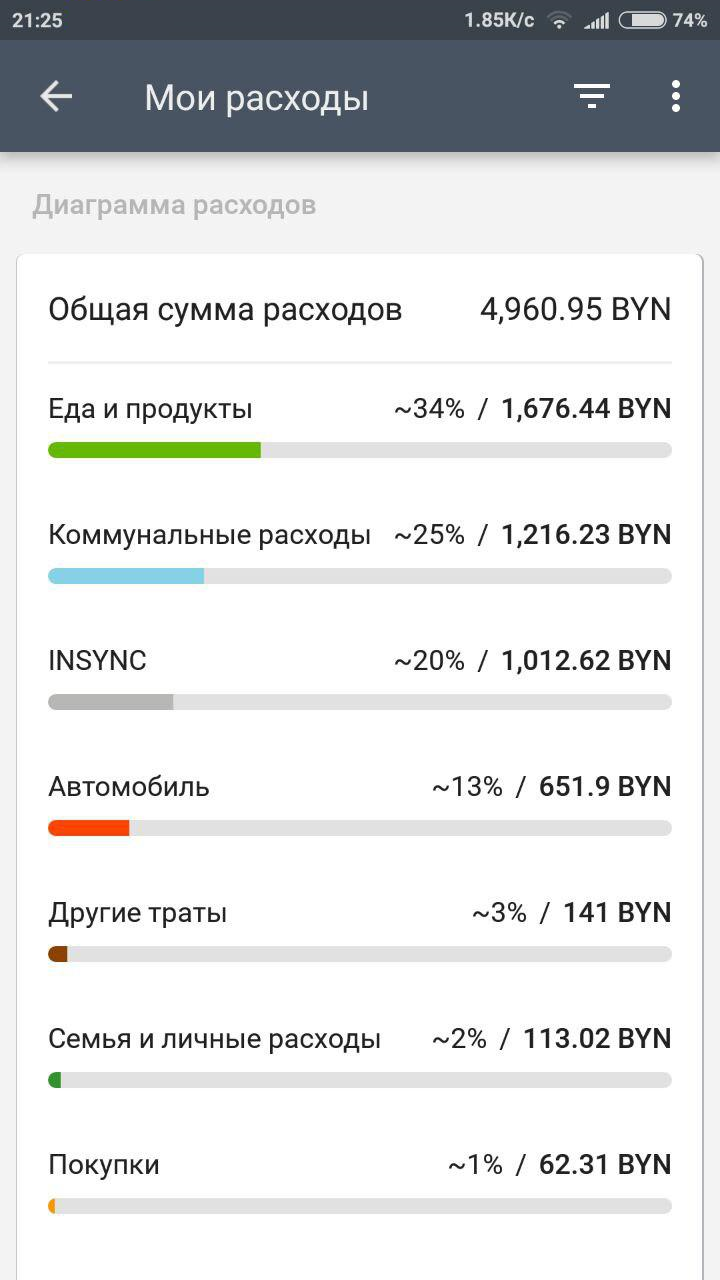
\includegraphics[scale=0.40]{1_2_alfabank.png}
    \caption{Статистика расходов по категориям приложения <<INSYNC.BY>>}
    \label{fig:analysis:analogues:alfabank}
\end{figure}

У описанного решения есть некоторые достоинства:
\begin{itemize}
    \item автоматизированный подсчет и учёт расходов;
    \item для категоризации расходов не требуются действия со стороны пользователя, достаточно производить оплату банковской картой.
\end{itemize}

Однако, несмотря на эти плюсы, у такого подхода есть ряд ощутимых недостатков:
\begin{itemize}
    \item приложения такого типа привязаны к конкретному банку и, соответственно, учитывают расходы только при платежах с карт этого банка;
    \item данный подход не учитывает наличные деньги;
    \item нет возможности самому контролировать категории расходов в силу того, что категории определяются автоматически исходя из типов заведений, в которых был произведен платеж;
    \item нет возможности определять категории доходов.
\end{itemize}

Описанный выше тип программных средств является быстрым решением, не требующим особых усилий для внедрения в повседневную жизнь, но в то же время не позволяет в полной мере вести учёт и анализ персонального бюджета.

Рассмотрим несколько различных приложений по учёту персонального бюджета

Первое из таких приложений -- <<Money Lover - Менеджер Расходов>> от разработчика Finsify.
Из преимуществ приложения можно выделить:
\begin{itemize}
    \item возможность иметь один аккаунт и приложение сразу на нескольких устройствах: компьютере, планшете и смартфоне;
    \item возможность установить лимит затрат и когда он будет исчерпан будут появляться уведомления, что больше тратить нельзя;
    \item в приложении присутствует большой выбор категорий по умолчанию, как и возможность создавать свои собственные;
    \item возможность генерировать отчёты о расходах и доходах за произвольный период;
    \item возможность управления долгами.
\end{itemize}

Однако большое количество возможностей неизбежно влечёт за собой такие недостатки, как перегруженность пользовательского интерфейса, наличие рекламных баннеров (рисунок~\ref{fig:analysis:analogues:money_lover}), которые закрывают до 15\% рабочего пространства, что осложняет быструю работу с приложением.
Стоит заметить необходимость регистрации в приложении для работы даже в режиме без соединения с сетью.
Кроме того, приложение достаточно плохо русифицировано, как это можно видеть в списке стандартных категорий (см. рисунок~\ref{fig:analysis:analogues:money_lover}б).

\begin{figure}[H]
    \centering
    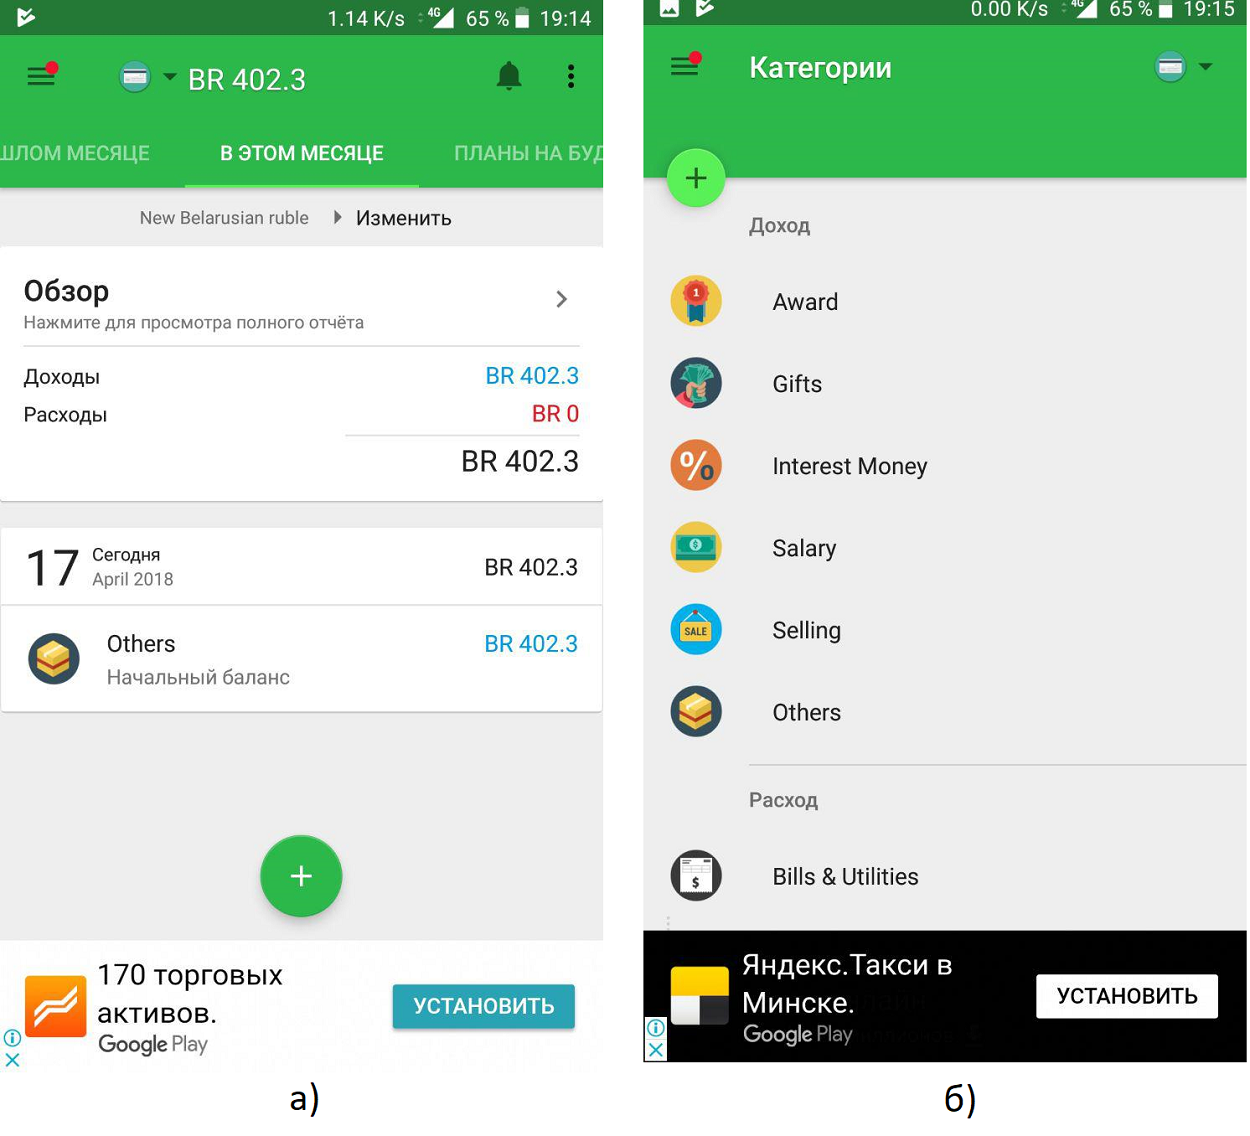
\includegraphics[scale=0.40]{1_2_money_lover.png}
    \caption{Некоторые экраны приложения <<Money Lover - Менеджер Расходов>>: а) -- главный экран; б) -- меню категорий}
    \label{fig:analysis:analogues:money_lover}
\end{figure}
